\section{Dynamical System: Analytic Solution}

To study the dynamics of the system, we need to consider the complete diffusion equation, along with the time dependent electric potential equation.

We consider

\begin{align}
\frac{\partial C_+}{\partial t} &= D_+ \left[\nabla^2 C_+ -  \nabla (C_+ \nabla \Psi) \right] , \\
\frac{\partial C_-}{\partial t} &= D_- \left[\nabla^2 C_- + \nabla (C_- \nabla \Psi) \right], \\
\nabla^2 \Psi &= -\kappa^2 \left(C_+ - C_- \right).
\label{eq:dynamic-system}
\end{align}

subject to the border condition 
\begin{align}
C_+(0, x) & = C^{SS}_+(x)\\
C_-(0, x) & =  C^{SS}_-(x)\\\
\Phi(0, x) &= \Phi^{SS}_+(x)\
\end{align}

where the super-script $SS$ indicates the steady state solution (See Ch. 2)%\ref{ch:2).

\subsection{Diffusion Only}

As a first approach to our problem, we evaluate the simpler diffusion-only problem



\begin{align}
\frac{\partial C_+}{\partial t} &= D_+ \nabla^2 C_+,\\
\frac{\partial C_-}{\partial t} &= D_- \nabla^2 C_-,
\label{eq:diffusion}
\end{align}

which in our limit (infinite plate) we can write as


\begin{align}
\frac{\partial C_s}{\partial t} &= D_s \frac{\partial^2 C_s}{\partial x^2},\\
\label{eq:diffusion-1d}
\end{align}

with $s=\pm$. The equation is subject to the following boundary conditions


\begin{align}
C_s(\delta, t) = C_b,\\
J_s(0,t) = D_s\frac{\partial C_s}{\partial x}\big|_{x=0} = r\delta_{+,s},
\label{eq:diffusion-bc}
\end{align}

where $J_s(x,t)$ is the flux for each species, which is non-zero only for the interacting species (copper, in our case). The initial condition for our system is

\begin{align}
	C_s(x, 0) = 0.
\label{eq:diffusion-bc}
\end{align}

First, we solve for $s=-$. Let 

\begin{align}
	\rho_-(x,t) &= C_-(x,t) - C_b,\\
	D_-\frac{\partial \rho_-}{\partial x}\big|_{x=0} &= J_-(0, t) = 0.
\end{align}

Considering the previous change of variables, we know need to solve the system

\begin{align}
\frac{\partial \rho_-}{\partial t} &= D_- \frac{\partial^2 \rho_-}{\partial x^2},\\
\label{eq:diffusion-1d}
\end{align}


We will solve this equation using the method of separation of variables. Let

\begin{align}
	\rho_-(x,t) = g_-(t)f_-(x)
\end{align}

We get the following two equations for $g_-(t)$ and $f_-(x)$


\begin{align}
	g_-'(t) + \lambda g_-(t) &= 0,\\
	f_-''(x) + \frac{\lambda}{D_-} f_-(x) &= 0.
\end{align}

$\lambda$ is a positive constant, due to border conditions. The solution to these equations are

\begin{align}
	g_-(t) =& g_{-}(0)e^{-\lambda t},\\
	f_-(x) =& F^1_{-,\lambda}\cos\qty{{\sqrt{\frac{\lambda}{D_-}} x}} + F^2_{-,\lambda}\sin\qty{\sqrt{\frac{\lambda}{D_-}} x},
\end{align}

where $F^1_{-,\lambda}$, $F^2_{-,\lambda}$ and $G_{-,0}$ are constants dependent on the parameter $\lambda$, which is yet to be determined. Border conditions \ref{eq:diffusion-1d} yield $B_{-,\lambda} = 0$. We get the general solution,


\begin{align}
	\rho_-(x,t) = \sum_{\lambda} A_\lambda e^{-\lambda t} \cos\qty{\frac{\lambda}{D_-} x},
\end{align}

where $A_{-,\lambda} = g_-(0)F^1_{-,\lambda}$. is a constant. Considering the border condition at $x=\delta$, we can determine the value of $\lambda$,


\begin{align}
	\rho_-(x=\delta,t) = \sum_{\lambda} A_\lambda e^{-\lambda t} \cos\qty{\frac{\lambda}{D_-} \delta} = 0.
	\label{bc-delta}
\end{align}

The only way (unless $A_{-,\lambda} = 0$, in which case we get the trivial solution) for equation \ref{bc-delta} to be zero is if we get

\begin{align}\nonumber
	\cos\qty{\sqrt{\frac{\lambda}{D_-}} \delta} = 0
\end{align}


\begin{align}
	\sqrt{\frac{\lambda}{D_-}} \delta = \frac{(2n+1)\pi}{2}.
\end{align}

Solving for $\lambda$,

\begin{align}
	\lambda  = \qty{\frac{(2n+1)\pi}{2\delta}}^2 D_-.
	\label{eq:lambda}
\end{align}

Replacing \ref{eq:lambda} into the general expression \ref{eq:general-expresion-rho},

\begin{align}
	\rho_-(x,t) = \sum_{n} A_n e^{-\qty{\frac{(2n+1)\pi}{2}}^2\frac{D_- t}{\delta^2}} \cos\qty{\frac{(2n+1)\pi}{2\delta} x}
	\label{bc-delta}
\end{align}

From initial condition \ref{bc-delta}, we have $\rho_- (x,0) = -C_b $, which in turn yields
\begin{align}
	-C_b = \sum_{n}A_n\cos\qty{\frac{(2n+1)\pi}{2\delta} x}.
	\label{eq:general-expresion-rho-t0}
\end{align}

Multiplying \ref{eq:general-expresion-rho-t0} by $\cos\qty{\frac{(2m+1)\pi}{2\delta^2} x}$ and integrating over the domain, 



\begin{align}
	-C_b\int_0^\delta \cos\qty{\frac{(2m+1)\pi}{2\delta} x} dx  = \sum_{n}A_n\int_0^\delta {\cos\qty{\frac{(2m+1)\pi}{2\delta} x}\cos\qty{\frac{(2n+1)\pi}{2\delta}x} } dx.
\end{align}


The integral on the LHS is simply
\begin{align}
	\int_0^\delta \cos\qty{\frac{(2m+1)\pi}{2\delta} x} dx = \qty{\frac{2\delta}{(2m+1)\pi}}\qty{\sin\qty{\frac{(2m+1)\pi}{2}}-\sin\qty{0}}.
\end{align}

Notice that

\begin{align}
	\sin\qty{\frac{(2m+1)\pi}{2}} = (-1)^m.
\end{align}


Therefore,

\begin{align}
	\int_0^\delta \cos\qty{\frac{(2m+1)\pi}{2\delta} x} dx = \frac{2\delta(-1)^m}{(2m+1)\pi}.
\end{align}

On the other hand, 

\begin{align}
	\int_0^\delta {\cos\qty{\frac{(2m+1)\pi}{2\delta} x}\cos\qty{\frac{(2n+1)\pi}{2\delta}x} } dx = \frac{\delta}{2}\delta_{m,n}.
\end{align}

The Fourier coefficients are thus

\begin{align}
	A_m = -\frac{4C_b}{\pi}\frac{(-1)^m}{(2m+1)}.
\end{align}


Plugging these coefficients into expression \ref{eq:general-expresion-rho-t0}

\begin{align}
	\rho_-(x,0) = -\frac{4C_b}{\pi} \sum_n \frac{(-1)^m}{(2m+1)}\cos\qty{\frac{(2m+1)\pi}{2\delta} x},
\end{align}

which in turn yields the concentration profile at time t=0

\begin{align}
	C_-(x,0) = C_b\qty{1-\frac{4}{\pi} \sum_n \frac{(-1)^m}{(2m+1)}\cos\qty{\frac{(2m+1)\pi}{2\delta} x}}.
\end{align}


From \ref{eq:general-expresion-rho-t0}, the time dependent solution for the concentration is

\begin{align}
	C_-(x,0) = C_b\qty{1-\frac{4}{\pi} \sum_n \frac{(-1)^m}{(2m+1)}\exp\qtys{-\qty{\frac{(2n+1)\pi}{2\delta}}^2\frac{D_- t}{\delta^2}}\cos\qty{\frac{(2m+1)\pi}{2} \frac{x}{\delta}}}.
	\label{eq:solution-diffusion}
\end{align}


\begin{figure}[htbp]
\centering
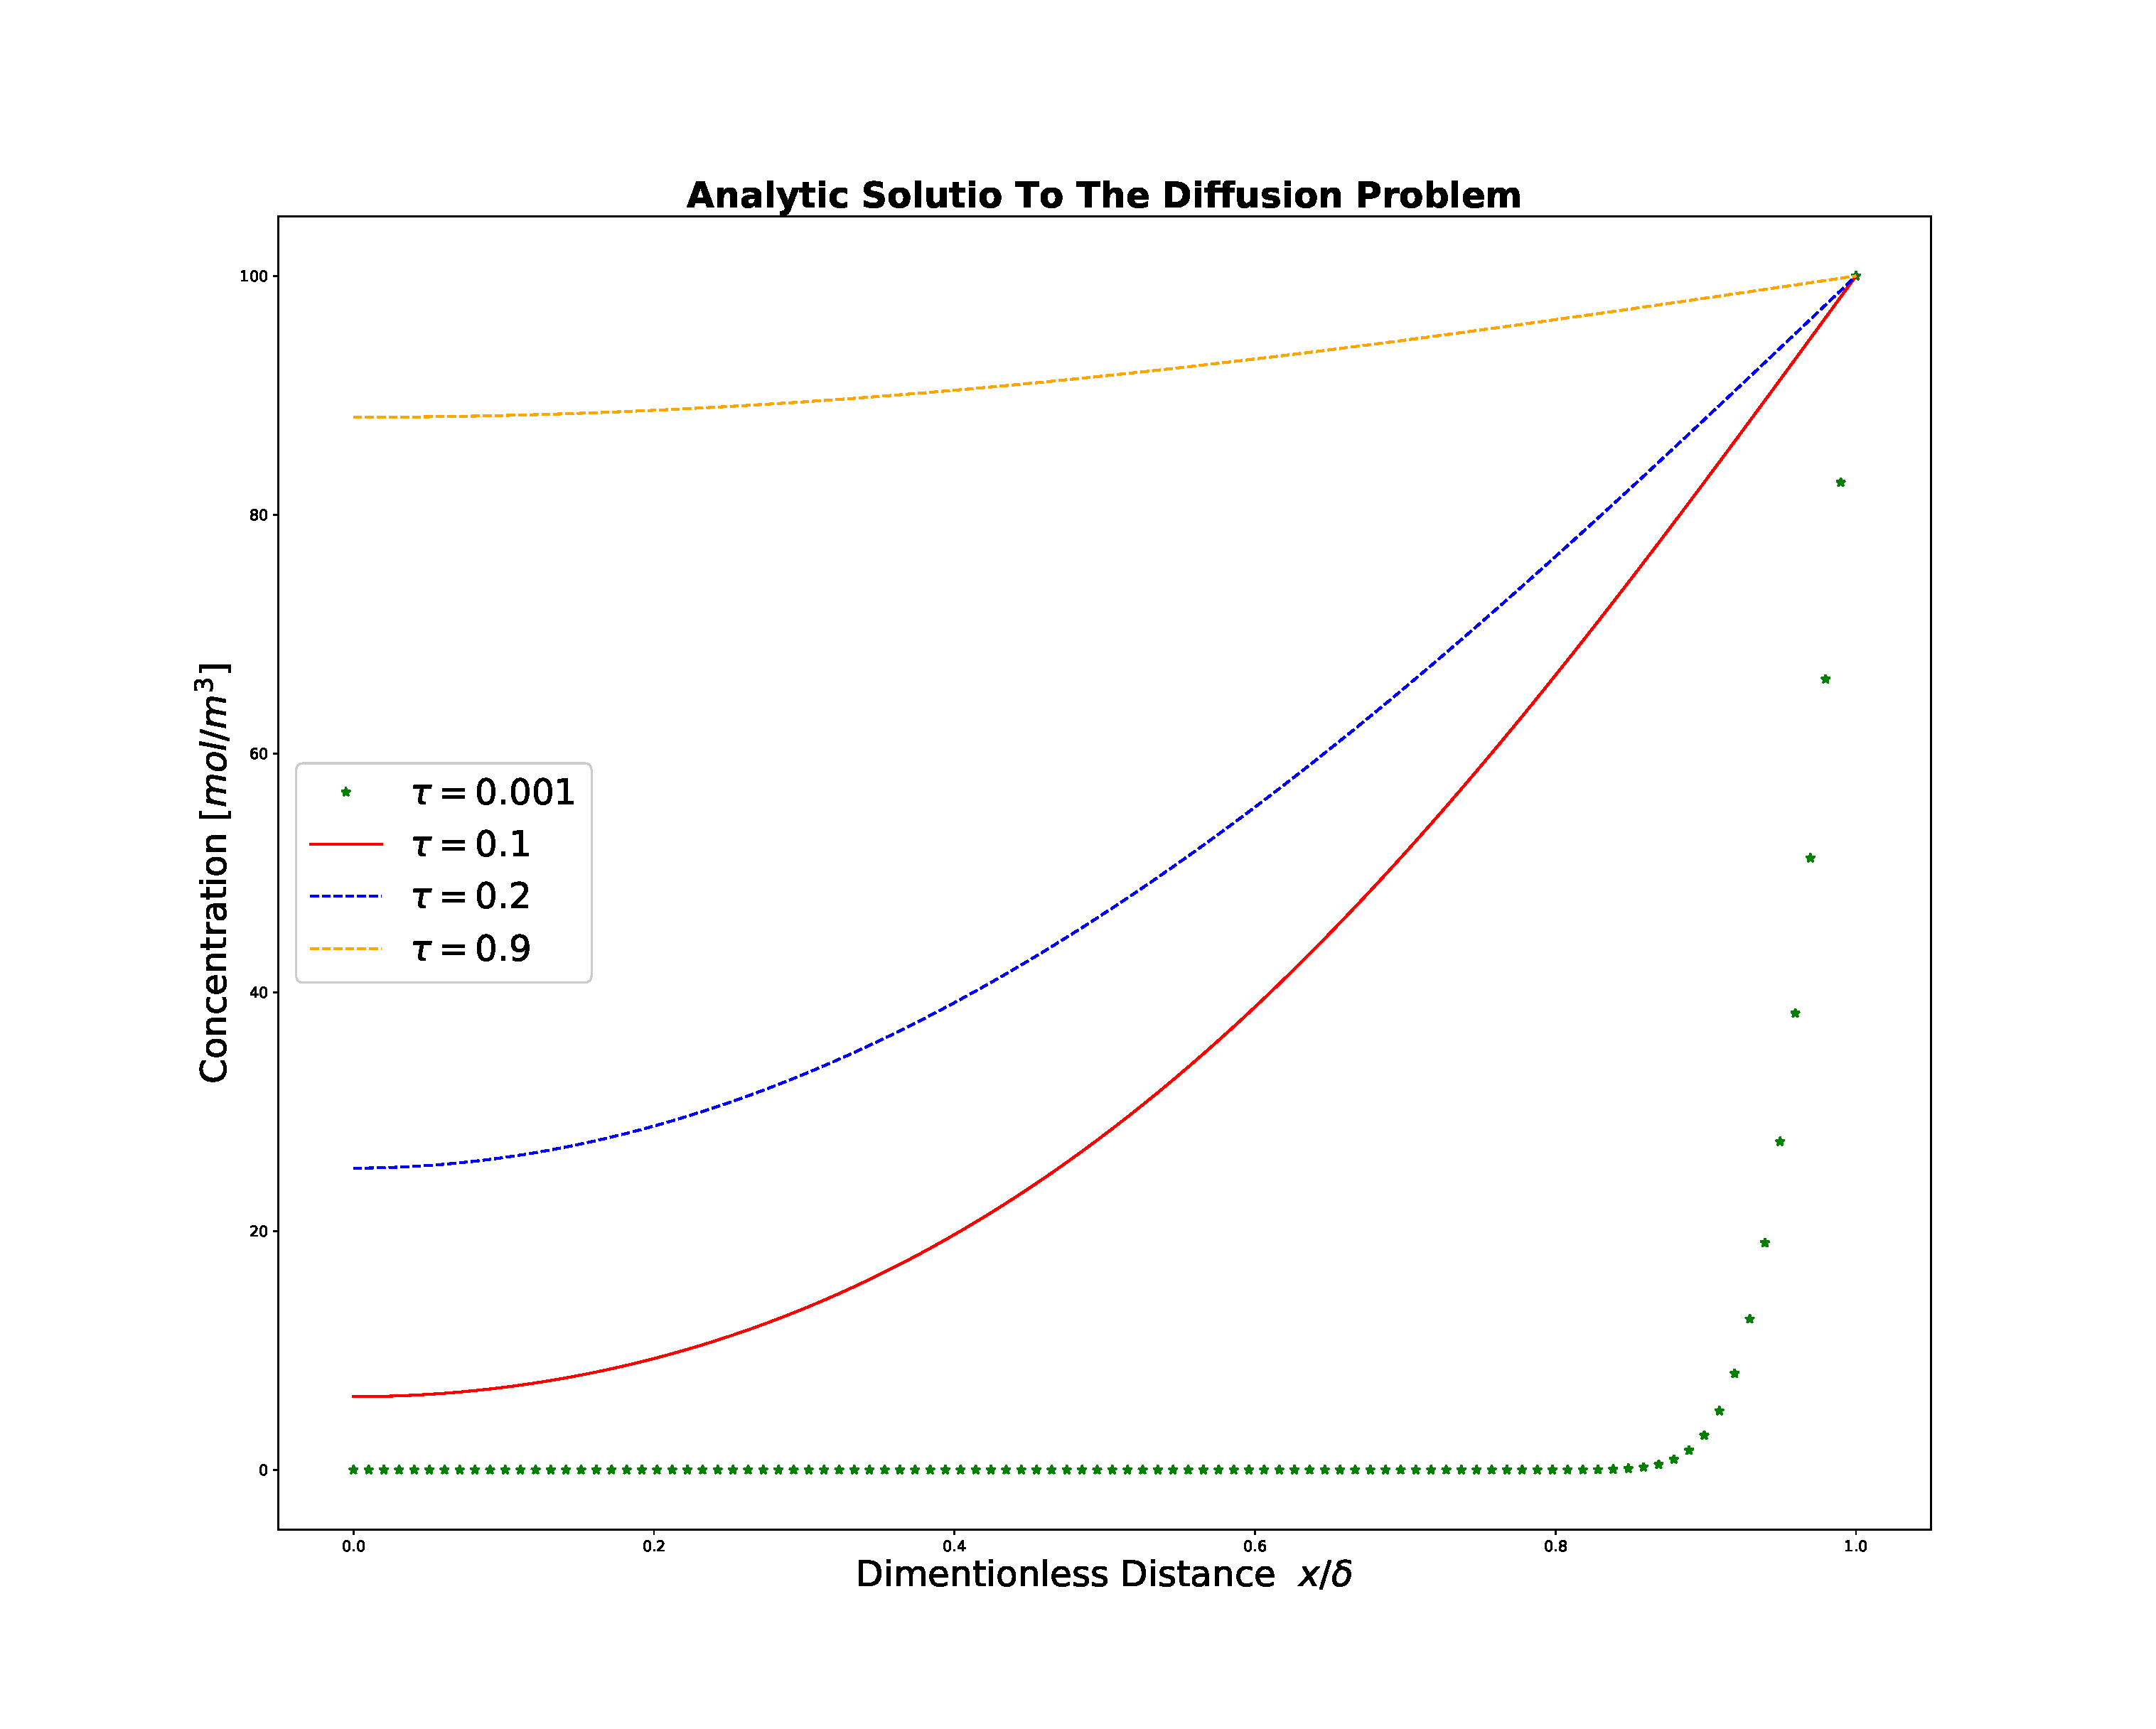
\includegraphics[width=\textwidth]{concentration-diffusiononly}
\caption{}
\label{fig:sub1}
\end{figure}

